\documentclass[a4paper, 11pt]{article}
\usepackage[utf8]{inputenc}
\usepackage[left=1in,right=1in,bottom=0.8in]{geometry}
\usepackage{enumitem}
\usepackage{graphicx}
\graphicspath{ {Figures/} }
\usepackage{float}
\usepackage[labelfont=bf]{caption}
\usepackage{fixltx2e}
\usepackage{caption}
\usepackage{amsmath}
\usepackage{capt-of}
\usepackage{minted}
\usepackage{tabu}
\let\svthefootnote\thefootnote

\title{\bf Experiment 3\\\vspace*{2mm} Combinatorial Circuits Using Quartus}
\author{\it Dhruv Ilesh Shah | 150070016}
\date{February 3, 2017}


\begin{document}
\maketitle
\section*{Overview}
In this lab, I have implemented the following combinatorial circuits on VHDL.
\begin{itemize}
	\item Two Bit Adder
	\item Two Bit Subtractor
	\item Priority Encoder
\end{itemize}
The code was compiled on Quartus Prime, and simulated using ModelSim. This was then uploaded to the {\em Krypton v1.1} 5M1270ZT144C5N CPLD-based board.

The codes and setup has been covered in section 1. Since the adder/subtractor have already been implemented by code in the previous labs, I shall skip the code details of those. The setup for the Priority Encoder, however, has been included. Section 2 includes the observations of the simulation and miscellaneous results.
\section{Setup}
For all the codes, Generic Testbench was used.

\subsection{Testing the Krypton Board}
The I/O pins on the Krypton board, and its basic functionality, was verified by running simple \texttt{svf} files on the board.

\subsection{Two Bit Adder}

The addition was carried out using $\oplus$ operations. Given input vectors $x_1x_0$ \& $y_1y_0$, we have the output $s_1s_0$ given by
\begin{equation}
\begin{split}
s_0 &= x_0 \oplus y_0 \\
s_1 &= x_1 \oplus y_1 \oplus x_0y_0
\end{split}
\end{equation}

Given below are the DUT definitions and code for the Adder.


\inputminted[linenos]{vhdl}{Submission/TwoBitAdder/DUT.vhd}
\hrule
\vspace*{2mm}
The code for the adder is as follows.


\inputminted[linenos]{vhdl}{Submission/TwoBitAdder/TwoBitAdder.vhd}
\hrule
\vspace*{2mm}

\subsection{Two Bit Subtractor}

The two bit subtractor is a simple 4-input, 2-output combinatorial circuit. After simplification of the terms, the logic can be given as.
\begin{equation}
\begin{split}
b_0 &= x_0 \oplus y_0 \\
b_1 &= x_1 \oplus y_1 \oplus \overline{x_0}y_0
\end{split}
\end{equation}
As for the implementation, I also 2 intermediate signals $s_1s_0$ defined as below.
\begin{equation}
\begin{split}
s_0 &= x_1 \oplus y_1 \\
s_1 &= \neg x_0 \cdot y_0
\end{split}
\end{equation}
And hence, the final output bit definitions look like:
\begin{equation}
\begin{split}
b_0 &= x_0 \oplus y_0 \\
b_1 &= s_0 \oplus s_1
\end{split}
\end{equation}

This can now be converted to VHDL code and simulated. In this experiment, I have used the \texttt{GenericTB} as testbench, which invokes a DUT entity, and hence the top-level entity would also need to be modified. Defining the DUT entity:

\inputminted[linenos]{vhdl}{Submission/TwoBitSubtractor/DUT.vhd}

\hrule
\vspace*{2mm}
Next up, we declare the entity \texttt{TwoBitSubtractor} and its functions. This has been shown below.

\inputminted[linenos]{vhdl}{Submission/TwoBitSubtractor/TwoBitSubtractor.vhd}

\hrule
\vspace*{2mm}
\subsection{Priority Encoder}

The 8x3 priority encoder is a combinatorial circuit that identifies the highest significance bit that is 1. This can be visualised as the truth table below, with {\em dont-cares}.
\begin{figure}[H]
\centering
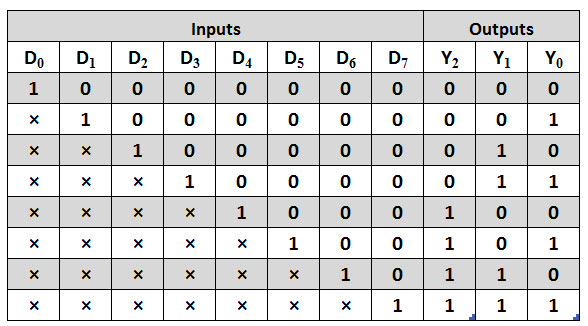
\includegraphics[scale=0.8]{PriorityEncoder_83}
\end{figure}

In addition to the 3 output bits, we also have an extra bit, say $N$, which is 1 if all the input bits are 0. For an input bit string $x_7x_6x_5x_4x_3x_2x_1x_0$, the output bit string $s_2s_1s_0N$ can be given by the relations
\begin{equation}
\begin{split}
N &= \overline{x_7+x_6+x_5+x_4+x_3+x_2+x_1+x_0} \\
s_0 &= x_1\cdot\overline{x_0} + x_3\cdot\overline{x_2}\cdot\overline{x_1}\cdot\overline{x_0} + x_5\cdot\overline{x_4}\cdot\overline{x_3}\cdot\overline{x_2}
\cdot\overline{x_1}\cdot\overline{x_0} + \\
& \hspace*{5mm} x_7\cdot\overline{x_6}\cdot\overline{x_5}\cdot\overline{x_4}\cdot\overline{x_23}\cdot\overline{x_2}\cdot\overline{x_1}\cdot\overline{x_0}\\
s_1 &= x_2\cdot\overline{x_1}\cdot\overline{x_0} + 
x_3\cdot\overline{x_2}\cdot\overline{x_1}\cdot\overline{x_0} +
x_6\cdot\overline{x_5}\cdot\overline{x_4}\cdot\overline{x_23}\cdot\overline{x_2}\cdot\overline{x_1}\cdot\overline{x_0}+
\\ &\hspace*{5mm} x_7\cdot\overline{x_6}\cdot\overline{x_5}\cdot\overline{x_4}\cdot\overline{x_23}\cdot\overline{x_2}\cdot\overline{x_1}\cdot\overline{x_0}\\
s_2 &= x_4\cdot\overline{x_3}\cdot\overline{x_2}\cdot\overline{x_1}\cdot\overline{x_0}
+ x_5\cdot\overline{x_4}\cdot\overline{x_3}\cdot\overline{x_2}
\cdot\overline{x_1}\cdot\overline{x_0} + \\
& \hspace*{5mm} x_6\cdot\overline{x_5}\cdot\overline{x_4}\cdot\overline{x_23}\cdot\overline{x_2}\cdot\overline{x_1}\cdot\overline{x_0}+
+ x_7\cdot\overline{x_6}\cdot\overline{x_5}\cdot\overline{x_4}\cdot\overline{x_23}\cdot\overline{x_2}\cdot\overline{x_1}\cdot\overline{x_0}
\end{split}
\end{equation}
\vspace*{1cm}
The VHDL implementation of this circuit has been given below. First, we define the container entity \texttt{DUT} as follow.

\inputminted[linenos]{vhdl}{Submission/PriorityEncoder/DUT.vhd}
\hrule
\vspace*{2mm}
Next up, we have the main segment of the code, as given in the file \texttt{PriorityEncoder.vhd}

\inputminted[linenos]{vhdl}{Submission/PriorityEncoder/PriorityEncoder.vhd}
\hrule
\vspace*{2mm}

Another essential part of the implementation is the testbench. Instead of using a custom testbench for the process, I have modified and used the \texttt{Generic Testbench} for an 8x4 implementation. Below is the code for the testbench. Main changes were made in lines {\em 9 - 18}.

\inputminted[linenos]{vhdl}{Submission/PriorityEncoder/Testbench.vhd}
\hrule
\vspace*{2mm}

Another important step in the evaluation of the simulation is the \texttt{TRACEFILE}. For this, I used the Python script given below.

\inputminted[linenos]{python}{Submission/PriorityEncoder/generate_tracefile.py}
\hrule
\vspace*{3mm}

This marks the end of the setup etc. We will now run RTL and Gate-level simulations on these codes, before deploying it on hardware.
\section{Observations}
In this section, I shall display the results of the running RTL and Gate-level simulations on the above implementations. Screenshots have been attached for each part.
\subsection{Two Bit Adder}
Figures 1-3 show the results of the simulation.
\begin{figure}[H]
\centering
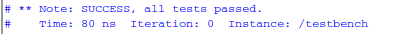
\includegraphics[scale=1]{Adder_Success}
\caption{Evaluation of the $2^4$ test cases for the Two Bit Adder.}
\end{figure}

\begin{figure}[H]
\centering
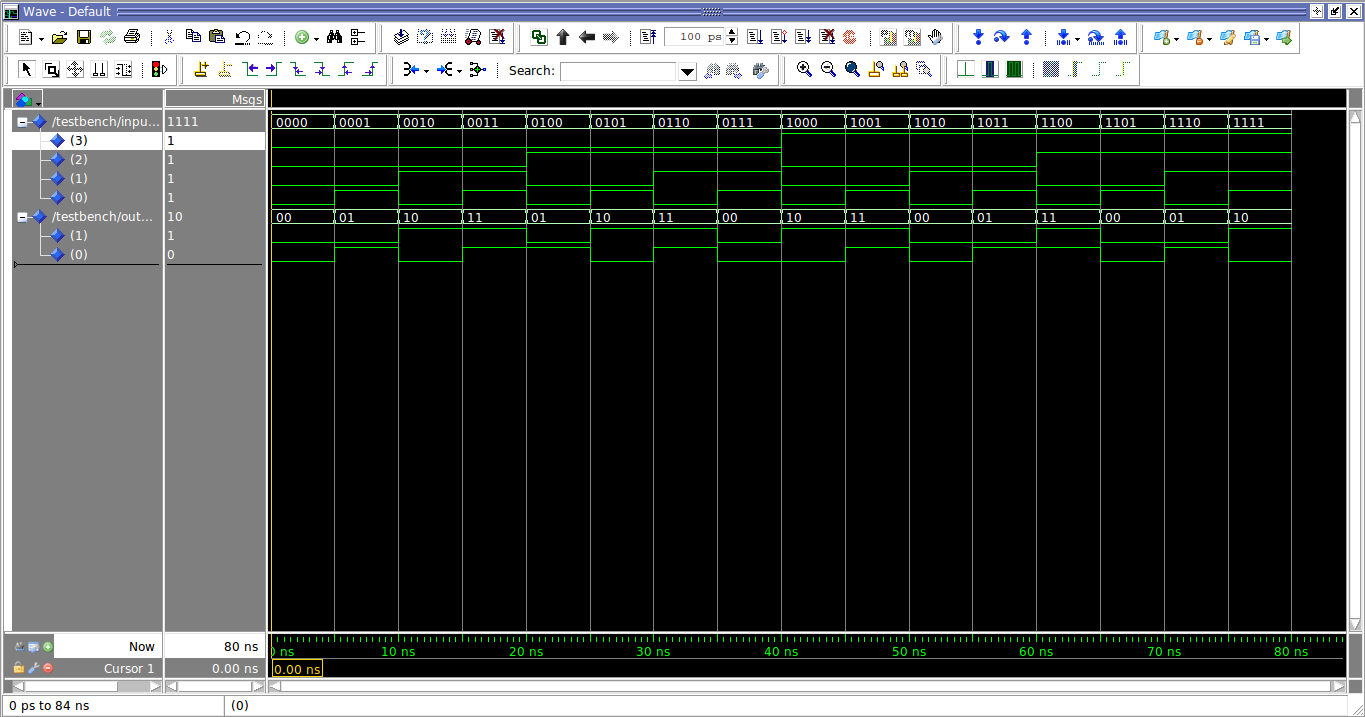
\includegraphics[scale=0.33]{Adder_RTL}
\caption{RTL Simulation of the Two Bit Adder}
\end{figure}

\begin{figure}[H]
\centering
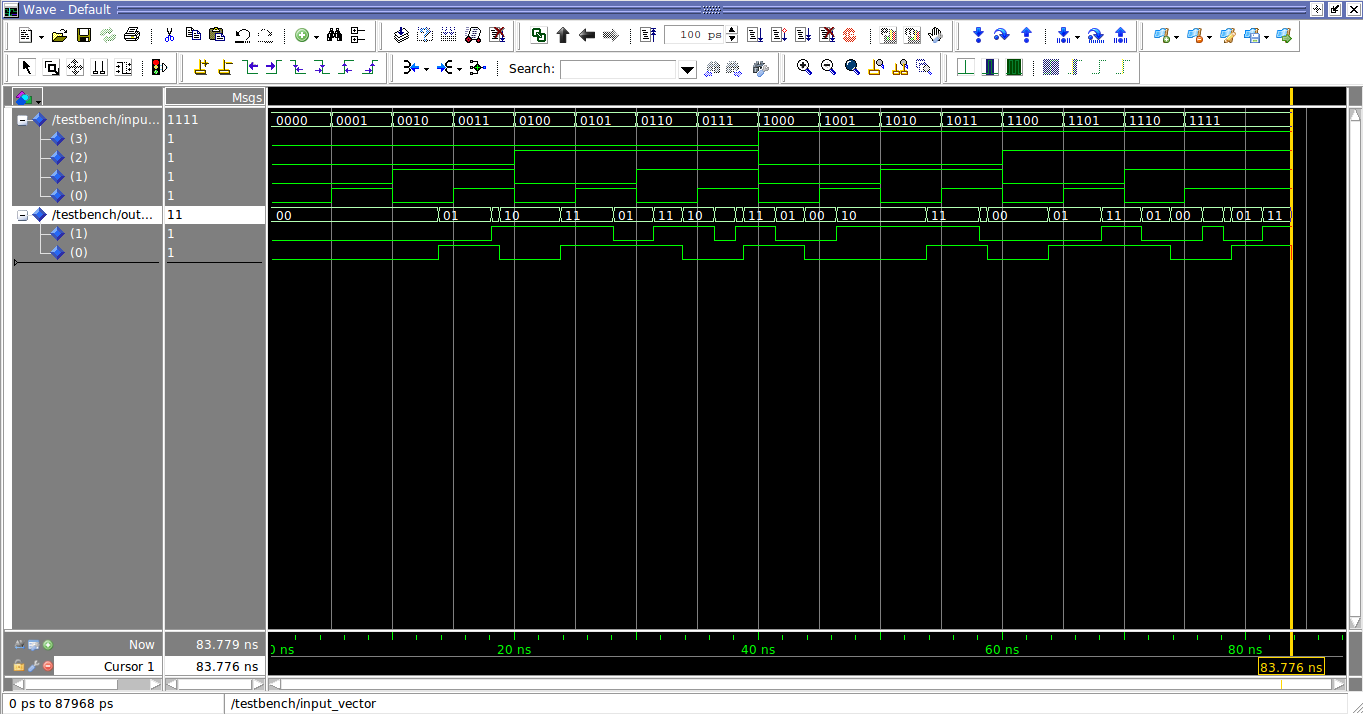
\includegraphics[scale=0.33]{Adder_Gate}
\caption{Gate-level Simulation of the Two Bit Adder}
\end{figure}

\subsection{Two Bit Subtractor}
Figures 4-6 show the results of the simulation.

\begin{figure}[H]
\centering
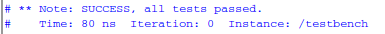
\includegraphics[scale=1]{Subtractor_Success}
\caption{Evaluation of the $2^4$ test cases for the Two Bit Subtractor.}
\end{figure}

\begin{figure}[H]
\centering
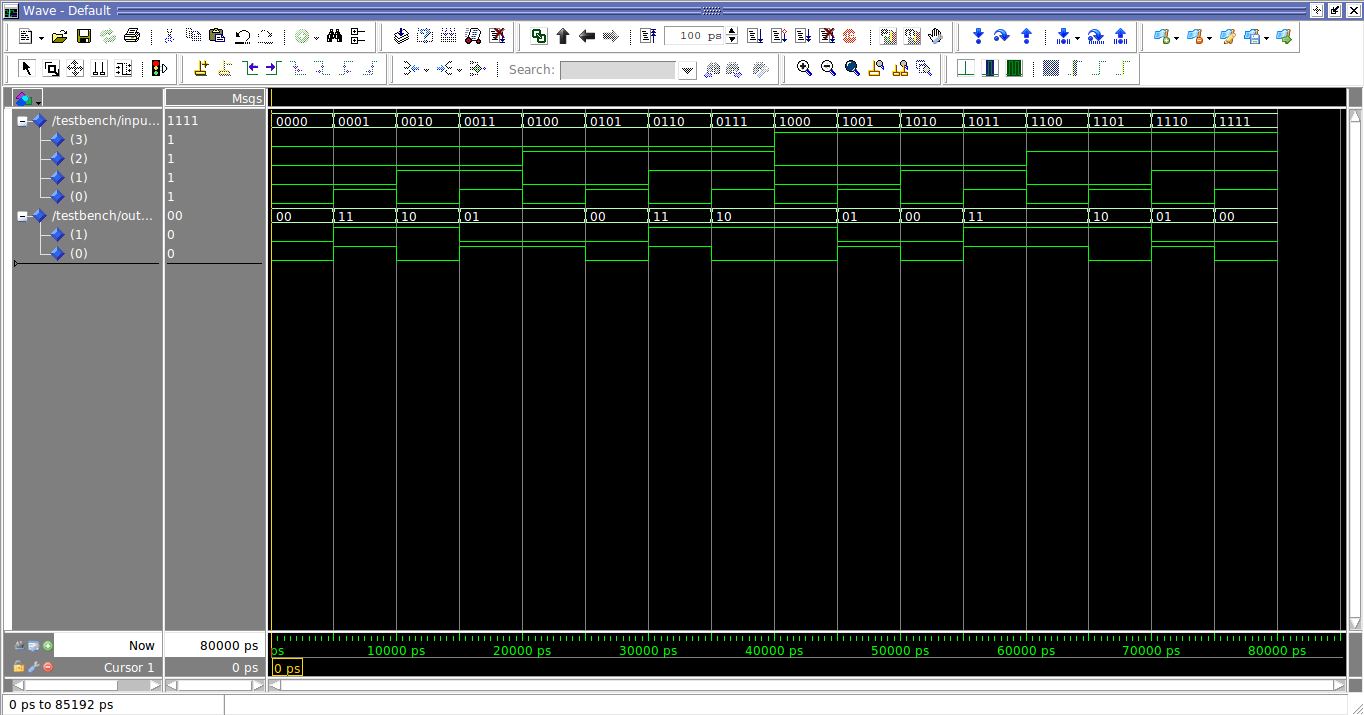
\includegraphics[scale=0.33]{Subtractor_RTL}
\caption{RTL Simulation of the Two Bit Subtractor}
\end{figure}

\begin{figure}[H]
\centering
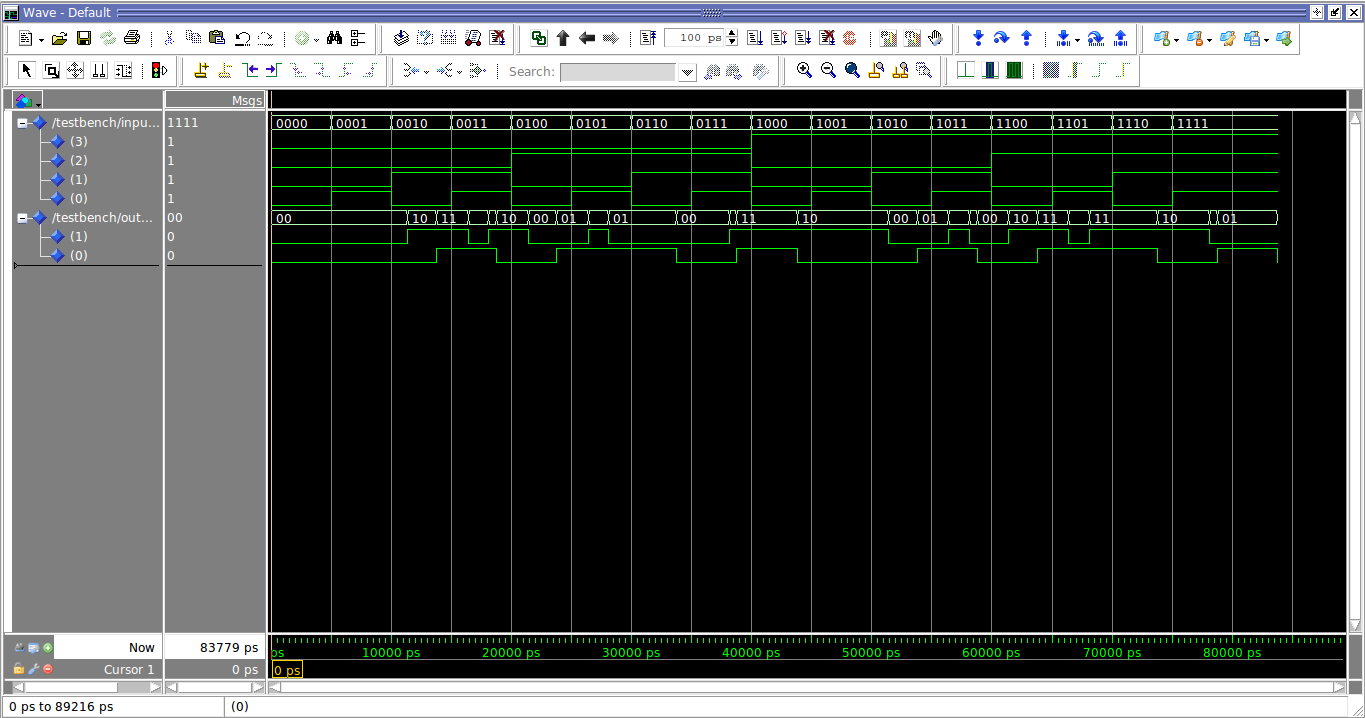
\includegraphics[scale=0.33]{Subtractor_Gate}
\caption{Gate-level Simulation of the Two Bit Subtractor}
\end{figure}

\subsection{Priority Encoder}
Figures 7-10 show the results of the simulation

\begin{figure}[H]
\centering
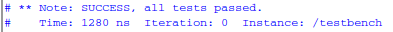
\includegraphics[scale=1]{PE_Success}
\caption{Evaluation of the $2^8$ test cases for the Priority Encoder.}
\end{figure}

\begin{figure}[H]
\centering
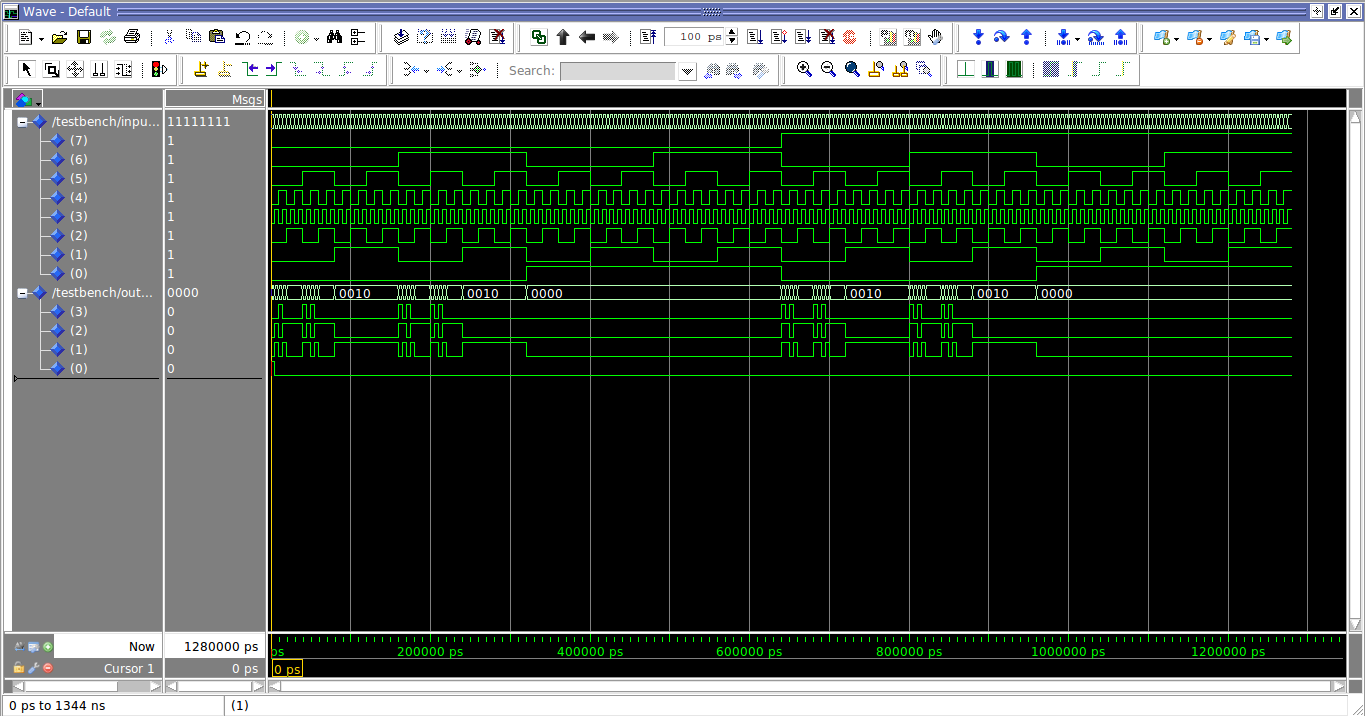
\includegraphics[scale=0.33]{PE_RTL}
\caption{RTL Simulation of the Priority Encoder}
\end{figure}

\begin{figure}[H]
\centering
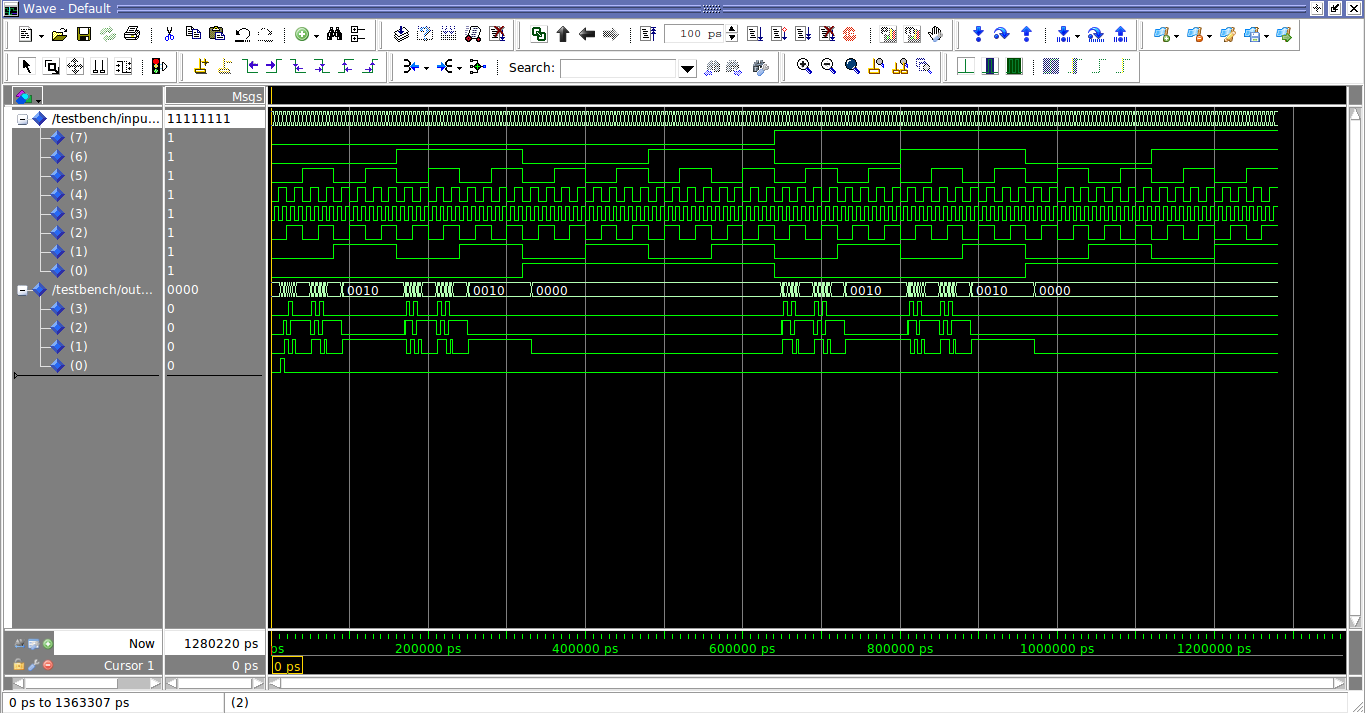
\includegraphics[scale=0.33]{PE_Gate}
\caption{Gate-level Simulation of the Priority Encoder}
\end{figure}

\begin{figure}[H]
\centering
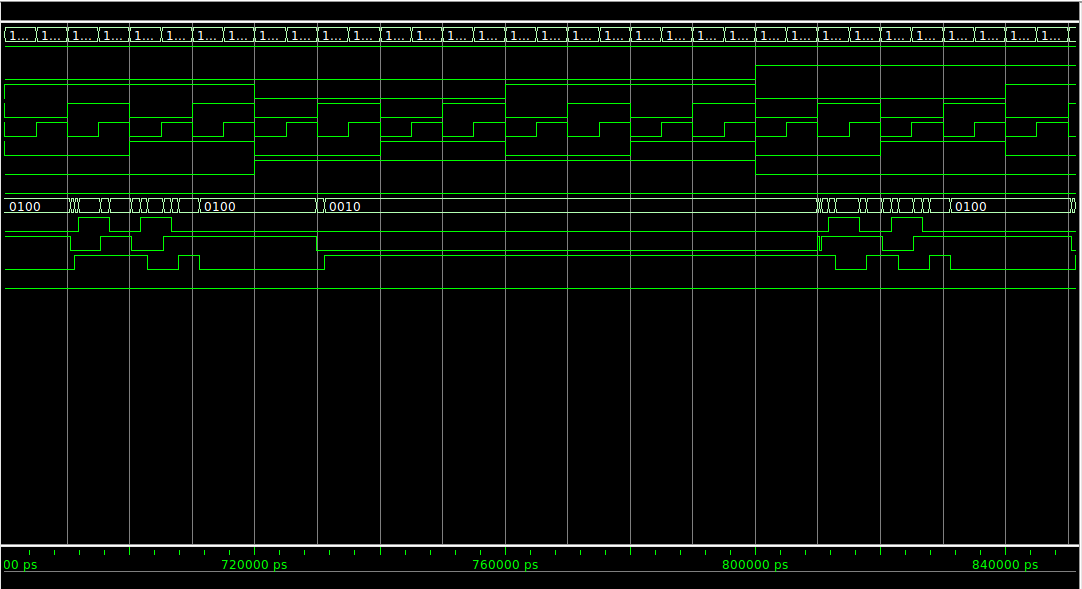
\includegraphics[scale=0.42]{PE_Gate_Zoomed}
\caption{Gate-level Simulation of the Priority Encoder, 760ns - 850ns}
\end{figure}

\section*{Conclusion}
We observe that the designs work well in the RTL simulations, but not in Gate level simulations. The gate level simulation emulated the gate delays, as they would exist in real hardware, and hence demonstrate a crucial bottleneck of the device. For ideal performance, the time between states should be increased so that the transient outputs can settle. Once this is done, the implementation can be uploaded on the CPLD for required purposes.

\end{document}
